% -*- TeX-master: "master.tex" -*-
\section{Introduction}

Two important questions in physics:
\begin{itemize}
\item What is matter made of?
  \begin{itemize}
  \item What are the elementary constituents?
  \end{itemize}
\item How do the elementary constituents interact?
  \begin{itemize}
  \item What are the forces and dynamics in Nature?
  \end{itemize}
\end{itemize}

Most popular media focus on the first question. In Fermilab's ``search for the top quark'', or the LHC ``quest for the Higgs boson'', focus is placed on the excitement of discovering new forms of matter.

This is fun, but what is really exciting is not garnering a new trophy, but in what the existance of these new particles implies for the second question --- what new dynamics must exist that this new particle can help reveal?

\subsection{The matter}
\begin{itemize}
\item Hydrogen:
  \begin{figure}[H]
    \centering
    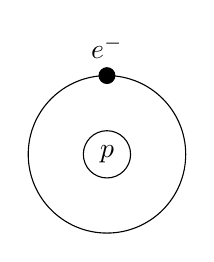
\begin{tikzpicture}{scale=1.5}
      \draw (0,0) circle [radius=0.3] node {$p$};
      \draw (0,0) circle [radius=1.0];
      \filldraw (0,1.0) circle [radius=0.1]
      node [yshift=1em] {$e^-$};
    \end{tikzpicture}
    \caption{Hydrogen Atom}
    \label{fig:hydrogen}
  \end{figure}
  A visualization is in fig~\ref{fig:hydrogen} Some properties of hydrogen:
  \begin{gather*}
    \text{Radius: } r_e\approx \SI{1}{\angstrom}\\
    \text{Binding Energy: }\SI{13}{\eV}
  \end{gather*}
  The unit of the binding energy is an Electron-Volt, which is what we will use for all energies for the duration of these notes.
  \begin{definition}[Electron-Volt]
    The electron volt is defined as the kinetic energy of an electron accelerated across a 1V potential, the usual SI unit prefixes can be applied such that 1keV=$10^3$eV, 1MeV=$10^6$eV etc.
  \end{definition}
\item Electron
  \begin{gather*}
    \text{Mass: } m_e= 0.511\text{ MeV}\\
    \text{Charge}=-1\\
    \text{Spin}=\frac12
  \end{gather*}
\item Proton
  \begin{gather*}
    \text{Mass: } m_p= 938\text{ MeV}\approx 1\text{ GeV}\\
    \text{Charge}=+1\\
    \text{Spin}=\frac12
  \end{gather*}
  \item Neutron
  \begin{gather*}
    \text{Mass: } m_n= m_p+1.3\text{ MeV}\approx m_p\\
    \text{Charge}=0\\
    \text{Spin}=\frac12
  \end{gather*}
  \item Deuterium is a Hydrogen with a neutron
\end{itemize}

\paragraph{Sizes}
\begin{itemize}
\item The electron is effectively a point
\item The nucleons, which are protons and neutrons have a ``radius'' of $\sim 10^{-15}$m, which is given the name of $1$fm, a ``Fermi'' or femtometer, which is notably less than the scale of hydrogen
\end{itemize}

\subsection{Forces in play:}
\begin{itemize}
\item Gravity $\sim$ negligible:
  \begin{align*}
    F=G_N\frac{m_p m_e}{r^2}
  \end{align*}
\item Electric:
  \begin{align*}
    F=\frac{e^2}{4\pi}\frac{Q_p Q_e}{r^2}
  \end{align*}
\item Strong --- Binds nucleons into nuclei
\item Weak --- Causes nuclear ``beta'' decay, and fusion
\end{itemize}

\subsection{Beta ($\beta$) decay}
A Process described by:
\begin{align*}
  n\to p+e^{-}+\bar{\nu}_e
\end{align*}
Where $\bar{\nu}_e$ is an anti-electron neutrino. This process has a lifetime $\tau$ of $\~14$ minutes.

Note that $m_n-m_p>m_e$

\paragraph{Q/ Why doesn't deuterium decay?} In short, conservation of energy, since $2m_p+m_e+m_{\nu_e}=1877.05$MeV, however, the mass of deuterium is $m_d=1876.64$. The masses are not large enough to allow for this decay:
\begin{figure}[H]
  \centering
  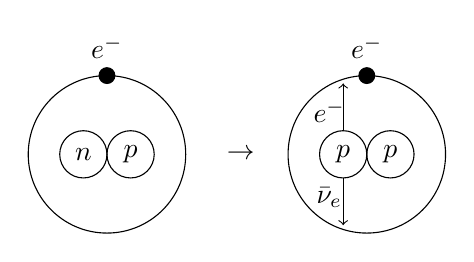
\begin{tikzpicture}
    \draw (0,0) circle [radius=0.3] node {$n$};
    \draw (0.6,0) circle [radius=0.3] node {$p$};
    \draw (0.3,0) circle [radius=1.0];
    \filldraw (0.3,1.0) circle [radius=0.1]
    node [yshift=1em] {$e^-$};
    \node at (2.0,0) {$\cancel{\rightarrow}$};
    \draw (3.3,0) circle [radius=0.3] node {$p$};
    \draw (3.9,0) circle [radius=0.3] node {$p$};
    \draw (3.6,0) circle [radius=1.0];
    \filldraw (3.6,1.0) circle [radius=0.1]
    node [yshift=1em] {$e^-$};
    \draw[->] (3.3,-0.3) to (3.3,-0.9) node [yshift=1em] {\hspace{-1em}$\bar{\nu}_e$};
    \draw[->] (3.3,0.3) to (3.3,0.9) node [yshift=-1em] {\hspace{-1em}$e^{-}$};
  \end{tikzpicture}
  \caption{Theoretical Deuterium Decay}
\end{figure}

\paragraph{Neutrinos and $\beta$ decay}
The other interesting story of $\beta$ decay is regarding the neutrino. In 1930, Chadwick observed the decay of tritium: $^3$H $\to\ ^3$He$+e^-$. Strangely, the $e^-$ was \emph{not} monoenergetic, as conservation of energy and momentum would require. This was catastrophic, and confronted with experimental evidence, many were prepared to throw out energy conservation. Pauli proposed a ``desperate remedy'' that some invisible particle must be carrying the energy away. Fermi's theory of weak interactions described this particle as a ``neutrino'' (little neutral one), and successfully described $\beta$ decay.

\textbf{Note}: The neutrino in $\beta$ decay was later found to be an antiparticle.

\begin{itemize}
\item Neutrinos then can be added to our list of ``matter''
  \begin{align*}
    \SI{0.01}{\eV}\leq m_{\nu_e}\leq\SI{1.4}{\eV}
  \end{align*}
  A consequence of this mass is that we can take neutrinos to be kinematically massless.
\end{itemize}

\subsection{Antiparticles}
Every particle has an antiparticle with opposite quantum numbers, but identical mass and spin:
\begin{itemize}
\item The electron $e^-$ has the positron $e^+$
\item The proton $p$ has the antiproton $\bar{p}$
\item The neutron $n$ has the antineutron $\bar{n}$
\item And the neutrinos $\nu$ have the antineutrinos $\bar{\nu}$ as we have seen
\end{itemize}
These (specifying the electron neutrino and its antiparticle) compose $\sim100\%$ of all the \textbf{observed} matter in the universe, though are only $5\%$ of the total matter.

Up to this point we have used chemistry and nuclear physics, particle physics picks up at the next level of depth.

\subsection{Quarks}
As it turns out, the proton and neutron are \textbf{not} fundamental.

If you perform a Rutherford-like scattering experiment at large energies (short distance), you find that protons and neutrons are composed of 3 hard spheres, called ``constituent quarks''

In fact, we go a bit deeper and find:
\begin{itemize}
\item The up quark $u$ and the up antiquark $\bar{u}$
\item The down quark $d$ and the down antiquark $\bar{d}$
\end{itemize}

These were ``predicted'' by Gell-Mann and Zweig as an explanation for apparent relationships between other particles, but we are getting ahead of ourselves.

The new particles we can add to our list of matter is:

\begin{itemize}
\item Up quark
  \begin{gather*}
    \text{Mass: } m_u= 4\text{ MeV} \ll m_p\\
    \text{Charge}=+\frac23\\
    \text{Spin}=\frac12
  \end{gather*}
\item Down quark
  \begin{gather*}
    \text{Mass: } m_d= 7\text{ MeV} \ll m_p\\
    \text{Charge}=-\frac13\\
    \text{Spin}=\frac12
  \end{gather*}
\end{itemize}
Note the odd fractional charge that both of these quarks have.

We can then think of $p,\bar{p}$ and $n,\bar{n}$ as:
\begin{figure}[H]
  \centering
  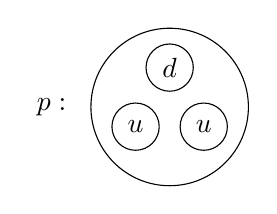
\begin{tikzpicture}
    \node at (0,0) {$p:$};
    \draw (1.500, 0.00) circle (1.0);
    \draw (1.500, 0.50) circle (0.3) node {$d$};
    \draw (1.067,-0.25) circle (0.3) node {$u$};
    \draw (1.933,-0.25) circle (0.3) node {$u$};
  \end{tikzpicture}
  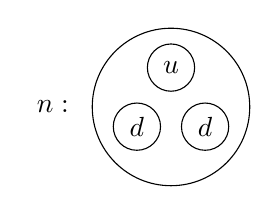
\begin{tikzpicture}
    \node at (0,0) {$n:$};
    \draw (1.500, 0.00) circle (1.0);
    \draw (1.500, 0.50) circle (0.3) node {$u$};
    \draw (1.067,-0.25) circle (0.3) node {$d$};
    \draw (1.933,-0.25) circle (0.3) node {$d$};
  \end{tikzpicture}
  \\
  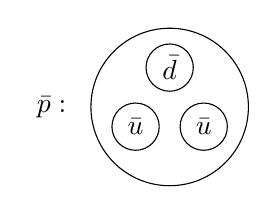
\begin{tikzpicture}
    \node at (0,0) {$\bar{p}:$};
    \draw (1.500, 0.00) circle (1.0);
    \draw (1.500, 0.50) circle (0.3) node {$\bar{d}$};
    \draw (1.067,-0.25) circle (0.3) node {$\bar{u}$};
    \draw (1.933,-0.25) circle (0.3) node {$\bar{u}$};
  \end{tikzpicture}
  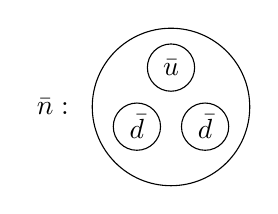
\begin{tikzpicture}
    \node at (0,0) {$\bar{n}:$};
    \draw (1.500, 0.00) circle (1.0);
    \draw (1.500, 0.50) circle (0.3) node {$\bar{u}$};
    \draw (1.067,-0.25) circle (0.3) node {$\bar{d}$};
    \draw (1.933,-0.25) circle (0.3) node {$\bar{d}$};
  \end{tikzpicture}
  \caption{Protons and Neutrons as Quarks}
\end{figure}

\subsection{Beta Decay Again}
We should revisit $\beta$ decay in terms of the constituent quarks of protons and neutrons. We instead see the process as:
\begin{figure}[H]
  \centering
  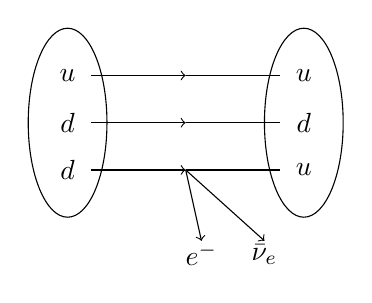
\begin{tikzpicture}
    \draw (0,0) ellipse (0.5 and 1.2);
    \node at (0, 0.6) {$u$};
    \node at (0, 0.0) {$d$};
    \node at (0,-0.6) {$d$};
    \draw (3,0) ellipse (0.5 and 1.2);
    \node at (3, 0.6) {$u$};
    \node at (3, 0.0) {$d$};
    \node at (3,-0.6) {$u$};
    \draw[->] (0.3, 0.6) to (1.5, 0.6);
    \draw[-]  (1.5, 0.6) to (2.7, 0.6);
    \draw[->] (0.3, 0.0) to (1.5, 0.0);
    \draw[-]  (1.5, 0.0) to (2.7, 0.0);
    \draw[->] (0.3,-0.6) to (1.5,-0.6);
    \draw[-]  (1.5,-0.6) to (2.7,-0.6);
    \draw[->] (1.5,-0.6) to (1.7,-1.5) node [yshift=-0.5em] {$e^-$};
    \draw[->] (1.5,-0.6) to (2.5,-1.5) node [yshift=-0.5em] {$\bar{\nu}_e$};
  \end{tikzpicture}
  \caption{$\beta$ decay in terms of quarks}
  \label{fig:beta}
\end{figure}
Thus we can describe the Fermi weak interaction in terms of quarks:
\begin{figure}[H]
  \centering
  \begin{tikzpicture}
    \begin{feynhand}
      \vertex (a) at (0,0) {$d$};
      \vertex (i) at (1.5,0);
      \vertex (b) at (3,0) {$u$};
      \vertex (e) at (3,1.5) {$e^-$};
      \vertex (n) at (3,-1.5) {$\bar{\nu}_e$};
      \propag[fer] (a) to (i);
      \propag[fer] (i) to (b);
      \propag[fer] (i) to (e);
      \propag[antfer] (i) to (n);
    \end{feynhand}
  \end{tikzpicture}
  \caption{``Four-Fermion'' Fermi Interaction}
  \label{fig:fermi}
\end{figure}

Thus so far, our ``Standard Model'' looks just like:
\begin{gather*}
  \pmqty{u\\d}\\
  \pmqty{\nu_e\\e}
\end{gather*}

However, there is still more to come!

